\chapter{Introduction}
\label{ch:introduction}

Put 15 in a four-bit register and add 1. The register now contains 0. Put the
same two values in wider registers and the result may be 16. Ask an operation
to keep a carry bit, and another part of the state changes as well. Ask it to
store the result, and addresses, byte order, and possible failure enter the
story. The written symbol (+) did not change. The machine around it did.

An instruction set makes these choices precise. It says which values exist,
where they live, how instruction bytes are decoded, which parts of state an
operation reads and writes, how control moves, and what happens when execution
cannot continue normally. A processor implements those rules. An assembler
gives them a readable spelling. A calling convention adds agreements between
separately written programs. These layers meet in ordinary code, but they are
not the same layer.

This book takes them apart and puts them back together.

\section{An old ambition with modern consequences}

The wish to make calculation mechanical is older than the electronic
computer. Binary arithmetic offered a spare alphabet. Stored-program designs
made instructions and data available to automatic control. Instruction-set
manuals then became contracts between hardware and software: compact enough
for programmers to use, detailed enough for implementations to share.

The present problem is not that those contracts have disappeared. It is that
our claims about programs now travel through more layers. A compiler rewrites
machine code. A superoptimizer searches for a shorter sequence. A binary
translator moves work between architectures. A solver reports that no
counterexample exists. A proof checker receives a certificate produced by yet
another program. At every boundary, a correct calculation can answer the
wrong question.

The superoptimizer made that tension explicit. Massalin searched instruction
sequences for the smallest implementation of a function in 1987.
\autocite{massalin1987} Later systems made the search broader and more
systematic, from peephole superoptimization to parallel hierarchical search.
\autocite{bansalaiken2006,lubodik2025} The modern question is no longer only
whether a machine can discover good code. It is what the word \emph{good}
means, whether the search covered the declared language, and what evidence a
skeptical reader can check afterward.

\begin{keyidea}[title={The book's central question}]
What must be defined, executed, related, and checked before a statement about
machine code deserves belief?
\end{keyidea}

This question includes ordinary correctness before it reaches optimization.
If two programs are said to agree, we need their state, inputs, outcomes, and
observation. If one is said to refine the other, we need the relation between
different machine states. If one is said to be minimal, we need the candidate
language and cost. The proof machinery comes last because it can only preserve
the meaning supplied to it.

\section{A machine small enough to finish}

We begin with an abstract instruction set called A0. It has fixed-width words,
eight registers, byte-addressed memory, a program counter, four condition
bits, and normal or exceptional outcomes. Its instructions move data, perform
integer arithmetic and logic, access memory, compare values, branch, and halt.

A0 is deliberately artificial. No hardware vendor must preserve its past, and
no software ecosystem depends on its encodings. We can therefore print its
whole relevant state and give every core instruction a complete rule. When an
example behaves unexpectedly, there is nowhere for a hidden architectural
custom to hide.

The point is not to design an ideal processor. A0 gives us a common language
for questions. What is a word? What counts as state? Does an operand name a
value, a location, or both? When do two addresses overlap? Does a branch read
registers directly or read condition state written earlier? What does it mean
for an execution to end?

After answering each question in A0, we ask it again of two real instruction
sets: x86-64 and RISC-V. Their differences then become informative rather than
bewildering. We already know the role that needs to be filled. We can inspect
how each architecture fills it.

\begin{sidebar}[title={Why invent A0 instead of starting with a real manual?}]
A real manual must serve compatibility, implementation, and reference needs.
Its definitions are distributed across chapters, modes, tables, and exception
rules. A0 lets the reader see one complete semantic dependency chain first.
The real manuals then become sources we can interrogate with precise
questions, not forests in which we hope to recognize familiar mnemonics.
\end{sidebar}

A0 also makes mistakes cheap. We can reverse byte order, omit a condition
write, or move a branch target by four bytes and immediately ask which claim
breaks. Those mutations become negative controls for the later executable
model. A teaching machine should make both the right rule and its nearest
wrong neighbors easy to inspect.

\section{Two companions, not two stereotypes}

RISC-V and x86-64 are often placed on opposite sides of a reduced-versus-
complex instruction-set contrast. The labels are historically useful, but
they cannot supply an instruction's meaning. They do not tell us which
register changes or how many bytes an encoding occupies. Nor do they say
whether arithmetic writes condition flags, which forms access memory, or what
a call does before an application binary interface (ABI) gives the stack a
role.

The book compares those dimensions directly. A base RISC-V instruction can
name a destination register separately from two sources. A selected x86-64
arithmetic form can use its destination as an input and also change condition
state. RISC-V commonly expresses memory traffic through load and store
instructions. Selected x86-64 arithmetic forms can name memory as an operand.
The base encoding structures differ. So do some of the special rules attached
to registers and operand widths.

None of these observations declares a winner. Each one creates a semantic
obligation. We have to record the right state, decode the right instruction
form, and compare the right outcomes. The labels RISC and CISC can summarize a family
resemblance after that work. They cannot perform it.

The real architectures in this book are also bounded slices. The name x86-64 will
never silently mean every historical mode, optional extension, privileged
operation, and processor timing table. The name RISC-V will never silently mean every
standard or proposed extension. Each load-bearing example will name the
instruction forms, state, source revision, privilege assumptions, and ABI
convention it uses.

\begin{warning}[title={Family labels are not causal explanations}]
Do not explain an effect by saying only that an architecture is RISC or CISC.
Name the actual dimension: operand role, instruction length, memory form,
condition state, address calculation, call mechanism, or extension boundary.
The label may summarize history after the rule is known.
\end{warning}

The sustained comparison has a second purpose. An abstraction that seems
natural after reading only one architecture may merely reproduce that
architecture's habits. A0 places condition bits in state, but RV64 branch
predicates remind us that control need not consume a separately stored flag.
A0 uses fixed four-byte encodings, but x86-64 reminds us that instruction
length can itself be a decoded result. The companions pressure-test the
foundation.

\section{From execution to a claim}

Suppose two short programs leave the same value in their designated output
register. Are they equivalent?

Perhaps. One may also change a scratch register. One may change condition
state that a later branch reads. One may touch memory, trap on an address, or
stop after a different number of instruction bytes. Agreement on the selected
output is a fact. Equivalence is a claim whose observation and preconditions
must say whether the other differences matter.

The book therefore constructs state before it studies optimization. A local
rewrite is not a relation between two lines of assembly alone. It is a
relation between their behaviors for every allowed starting state. If the
rewrite crosses architectures, equality is usually the wrong shape. The two
machines have different register names and condition state. We instead relate
their inputs and show that their executions produce related outputs.

The difference between a test and a proof begins here. Running both programs
on ten inputs may reveal an error. Passing ten inputs does not settle a claim
about every allowed state. For small domains we may enumerate all cases. For
larger finite domains we may ask a solver for a \keyterm{counterexample}: one
input on which the programs differ. If none exists, we must still ask what formula the solver received, which semantics
produced it, and what independently checkable evidence supports the result.

The machinery is valuable only after the statement is right. A perfect proof
of a formula about the wrong flags or a reversed byte order proves the wrong
thing with unusual confidence.

Consider two four-bit programs. Program $P$ adds 1 to register $r_0$ and
halts. Program $Q$ adds 1 to $r_0$, clears $r_1$, and halts. If the only
reported output is $r_0$, the programs agree on every input. If the caller
may inspect $r_1$, they do not. Neither conclusion is a correction to the
other. They answer different questions because they use different
observations.

Now give addition a carry output. On an initial $r_0=15$, both programs
leave 0 in $r_0$, but a version that forgets to update carry no longer agrees
with one that follows the full addition rule. A test that starts at $r_0=3$
will miss the defect. The boundary input 15 exposes it. This small example
contains the structure of much larger verification tasks: declare the input
set, execute a complete state transition, select an observation, and quantify
over every allowed start.

The order matters. If we first notice that the printed values of $r_0$
match, we may be tempted to name the programs equivalent and repair the
definition afterward. The book uses the reverse discipline. We decide what a
client may observe, then ask whether the two executions agree under that
observation. A claim is not a favorable output with a grander name.

\begin{definition}[title={Observation relative to a client}]
An observation is a declared function that extracts the parts of a machine
outcome a particular client may distinguish. Two outcomes agree for that
client when the observation returns the same result for both. Changing the
client may change the observation and therefore change the claim.
\end{definition}

\begin{figure}[htbp]
\centering
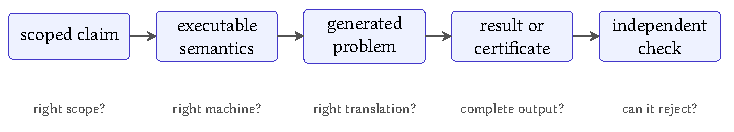
\includegraphics[width=0.98\textwidth]{figures/claim-evidence-chain}
\caption{A machine-backed claim crosses several trust boundaries. Each arrow
needs its own explanation and failure test.}
\figalt{A scoped claim leads through semantics, a generated problem, an artifact, and an independent check.}
\label{fig:claim-evidence-chain}
\end{figure}

Figure~\ref{fig:claim-evidence-chain} shows why a final green check is not
enough. The checker may faithfully validate an artifact for a generated
problem. The generator may faithfully encode executable semantics. Those
semantics may still omit a flag that the original claim meant to preserve.
Assurance accumulates only when every connection is identified.

\begin{example}[title={A correct proof of the wrong byte order}]
Suppose a generator reverses the weights used to join four memory bytes. A
solver and certificate checker may correctly establish every property of that
generated function. The result still does not prove a claim about A0
little-endian loads. The failure lies before the solver, at the connection
between the printed semantics and the generated problem.
\end{example}

\section{The two proofs}

Every load-bearing theorem in this book needs two forms of support. The reader
proof exposes the reason. It may use a width-four example, an invariant, a
case split, a short simulation, or a contradiction that can be reconstructed
at a blackboard. The machine proof covers the declared finite space through an
artifact and a checker that can reject damaged evidence.

Neither can replace the other. A solver log does not explain why a branch
rewrite works. A persuasive hand calculation does not cover every 64-bit
input. The hand argument tells us what the encoding should preserve. The
machine route tells us whether the industrial-size instance contains an
exception.

Computations keep a separate name. An exhaustive run can be valuable and
reproducible without carrying a proof certificate. The book states which kind
of evidence it has rather than promoting every successful command to the same
rank.

We also make the checker lose. A nearby false claim, mutated instruction,
damaged trace, or truncated certificate must be rejected for the expected
reason. This negative control cannot prove the original statement. It can show
that the route distinguishes at least one precise error from success.

The two proofs also fail differently. A reader argument may omit a case or use
an unstated premise. A machine route may encode the wrong operation, search an
incomplete candidate language, accept a damaged certificate, or lose the
provenance of its inputs. Placing them beside each other creates useful
friction. The hand proof tells us which invariant and controls to expect. The
machine result tells us where the friendly miniature stopped covering the
real finite domain.

\begin{proofkit}[title={\iconProofKit\ Three recurring proof shapes}]
Word and state laws often use a case split or direct algebra. Program
equivalence often uses an invariant or simulation across steps. Minimality
usually argues by contradiction: assume a cheaper candidate exists, encode
that existential claim, and refute every candidate in the declared language.
The shape of the proof follows the quantifier in the claim.
\end{proofkit}

\section{The route through the book}

\begin{figure}[htbp]
\centering
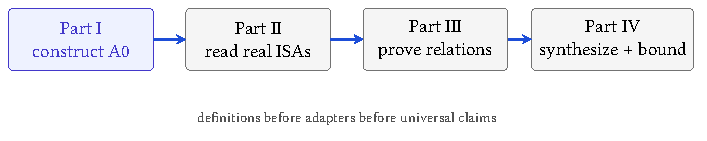
\includegraphics[width=0.95\textwidth]{figures/book-proof-route}
\caption{The curricular order follows the dependency order of the eventual
proofs. Later parts may not bypass a missing semantic layer.}
\figalt{Part I constructs A0, Part II reads real ISAs, Part III proves relations, and Part IV synthesizes and marks limits.}
\label{fig:book-proof-route}
\end{figure}

Part I constructs A0. Chapter 1 begins with words and the several meanings a
fixed pattern can receive. Chapters 2 through 5 add state, operands,
instructions, memory, programs, and control. By the end, the reader can execute
a small A0 program by hand and say exactly why each state change occurs.

Part II keeps one concept fixed while placing RISC-V and x86-64 beside it.
Encoding and decoding come first because instruction bytes and instruction
meaning are different objects. Data movement, addresses, arithmetic,
condition state, control transfer, procedures, stacks, and ABIs follow. The
comparison stays paired: we do not teach one architecture as normal and the
other as a collection of exceptions.

Part III asks what can be proved about programs. It develops observation,
equivalence, refinement, cross-ISA simulation, and candidate program languages.
It then asks about cost and \keyterm{minimality}, the claim that no cheaper
candidate exists. The proof system grows
from the semantics already on the page.

Part IV carries one scalar algorithm through A0, RV64, and x86-64. The final
chapter then marks the edge of the model: floating point, packed and vector
state, concurrency, privilege, virtual memory, self-modifying code, timing,
and leakage all require more structure than the scalar sequential core.

The order is an argument. First say what a machine step means. Then compare
real steps. Then relate programs. Then ask a finite artifact to support a
universal sentence.

The chapters are not independent essays. A byte-order proof in Chapter 4
depends on the word decomposition in Chapter 1. A trace in Chapter 5 depends
on the complete step in Chapter 3. A cross-ISA simulation in Chapter 12 will
depend on both real-ISA adapters from Part II. A minimality statement in
Chapter 13 will depend on all of those semantics plus a candidate language and
cost. The dependency chain prevents a solver formula from quietly becoming a
machine theorem.

\section{How to work through a chapter}

The book is meant to be used with pencil, terminal, and source manual near one
another. New material normally arrives in five passes. First comes an object
in ordinary language: a word, state, operand, instruction, trace, or relation.
Next comes a mathematical definition precise enough to settle boundary cases.
Then a small instance is executed or proved by hand. A real-architecture
comparison asks which parts survive contact with RV64 and x86-64. Only then
does an Axeyum route enlarge or check the claim.

Do not skip the hand execution because the code can run it. For a transition,
write the old state on the left and the new state on the right. Circle every
component the instruction reads. Mark every component it writes. State why
the untouched components remain unchanged. This practice catches omitted
state before a solver turns the omission into thousands of flawless but
irrelevant cases.

Proofs deserve a similar first pass. Before following symbols, identify the
quantifier. Is the claim about one execution, every word of a fixed width,
every state satisfying a premise, or every candidate below a cost bound? Then
identify the proposed reason: decomposition, invariant, simulation, or
contradiction. The details become easier to judge once the burden is visible.

\begin{proofkit}[title={\iconProofKit\ A six-question reading routine}]
For each load-bearing claim, ask:
\begin{enumerate}
\item What are the objects, and are their widths and state components fixed?
\item Which starting objects are allowed?
\item What outcome or observation is compared?
\item Is the claim about one case, a finite domain, or an unbounded family?
\item What is the human-scale reason it should hold?
\item What artifact, checker, and failing control cover the machine route?
\end{enumerate}
If one answer is missing, pause there. Later machinery cannot supply an
earlier definition.
\end{proofkit}

Exercises carry part of the exposition. The early ones rehearse a definition
on a new value. Middle exercises alter a premise or observation and ask which
conclusion survives. Later ones ask for a proof, a counterexample, or a small
checker. Some deliberately present an attractive false statement. Finding the
smallest state that breaks it is often more instructive than reading another
warning about hidden assumptions.

The figures also have jobs beyond decoration. A state diagram inventories
what must be preserved. An encoding diagram separates bit fields from their
decoded roles. A control-flow graph turns a program counter update into a
visible fork. When a figure seems obvious, try to redraw it from the adjacent
definition. Any edge or field that cannot be justified is a useful question
for the text or model.

Readers may choose different depths without changing the logical order. A
first course can execute A0 examples, study the paired ISA cases, and complete
selected reader proofs. A verification course can add every artifact and
negative control. An experienced compiler engineer may move quickly through
basic arithmetic but should resist skipping the observation and state
relations: those are where familiar optimization claims acquire exact scope.

\section{How Axeyum enters the argument}

Axeyum is the evidence stack used by the accompanying repository. It supplies
bit-vector expressions, solver routes, certificate machinery, and other
formal infrastructure. This book asks it to grow new architectural layers:
A0 execution, bounded real-ISA slices, decoders, state relations, and replay.
The software is introduced when a mathematical need appears rather than in a
detached command tour.

The first use is deliberately modest. A reader constructs one fixed-width
word, evaluates an operation, and asks whether a proposed identity has a
counterexample. The next layer constructs complete A0 states and observations.
Later layers execute instructions and traces, relate states from different
machines, generate solver problems, and check evidence. Each addition should
reuse the semantics already exercised by hand.

\begin{sidebar}[title={The four questions to ask of an Axeyum result}]
What exact statement entered the route? Which executable semantics generated
it? What artifact or model came back? Which independent program checked or
replayed the result, and what nearby false input did that route reject?
\end{sidebar}

The chapter sequence is not an Axeyum reference manual. Commands and interfaces may change;
the evidentiary questions should not. The repository guide pins the checkout,
build steps, route, and limitations used by each machine-backed object. A
reader interested only in the mathematics can follow the reader proofs. A
reader interested in trust can reproduce the machine route and attack its
controls.

At the current boundary, Axeyum has useful formal substrate but not the A0,
RV64, x86-64, and cross-ISA packages the full book requires. Planned examples
remain labeled as obligations until those packages and their controls run.
This prevents tutorial prose from becoming accidental evidence.

\section{What the ledger is for}

The project keeps a machine-readable record for its definitions, claims, and
unresolved obligations. Chapters take scope and evidence descriptions from
that record rather than inventing stronger wording in prose. Evidence files
carry raw digests. Checkers return failure when a claim, artifact, or control
does not meet its contract.

The ledger is not the subject of the first chapters. A reader should meet a
word before meeting its object record. They should understand a state
transition before meeting its formula. The record keeps the book honest when a
claim moves between prose, executable semantics, solver input, and checked
result.

Three distinctions in that record matter throughout the book. A definition
fixes vocabulary and creates an implementation obligation; it does not become
truer because software happens to represent it. A theorem makes a universal
claim and needs an argument that covers its stated domain. A computation
reports the result of a reproducible finite procedure. It may settle a bounded
question, find a witness, or expose a counterexample without pretending to be
a proof of something larger.

The printed artifact panels bind those distinctions to concrete evidence. An
identifier points to the record. The scope names widths, instruction forms,
starting states, observations, and cost assumptions. The route names the
generator or executor and the checker. The limitation says what the route
does not establish. A digest detects a changed file; it does not establish
that the file expresses the intended machine. That connection still needs
semantic review and controls.

\begin{keyidea}[title={Every chapter makes the same promise}]
The ordinary prose will say what an object means and why a claim should hold.
The formal statement will fix its scope. When machine evidence exists, the
artifact route will say how to reproduce and challenge it. When a required
route does not yet exist, the book will name the missing work instead of
borrowing certainty from a nearby calculation.
\end{keyidea}

This separation also lets the manuscript improve without rewriting its own
history. A missing executable layer can later be implemented and checked. A
computation can later gain a certificate. A false conjecture can be replaced
by its smallest counterexample. The prose must then change where the evidence
changes, but the reader never has to infer that a successful command silently
upgraded the kind of claim being made.

At present, the mature solver machinery is ahead of the architectural layers
this revised book requires. The missing work is stated plainly. Axeyum must
gain reusable A0 state and execution, source-pinned RV64 and x86-64 slices,
decoders, and cross-machine state relations before the later chapters can
claim semantics-backed ISA proofs. A handwritten bit-vector identity is not a
substitute for those layers.

That boundary is a useful place to begin. We know the machine we need to
construct, the two real systems against which it must answer, and the kinds of
evidence that would let a skeptical reader check the result. Chapter 1 starts
with the smallest object any of them can hold: one fixed-width word.
